In this section we will give an overall description of the main algorithms required in order enable Travlendar+ system to work as intended and to satisfy both functional and non functional requirements.
The following algorithms are explained with different methods, this allow us to focus on different details that must be described in different algorithms.

\section{Path calculation}
\label{sect:Path calculation}
	In order to compute optimal paths that include also sharing vehicles, not included into the set of possible travel means offered by \textit{Google Map APIs}, the system will have to implement some additional logic. We will handle the sharing vehicles option as an additional possible public travel mean, for example an user could want to take a bike in sharing instead of taking the subway.\\
The algorithm that implements this functionality will follow the behavior explained in the pseudo-code below:
\begin{figure}[H]
\begin{center}
		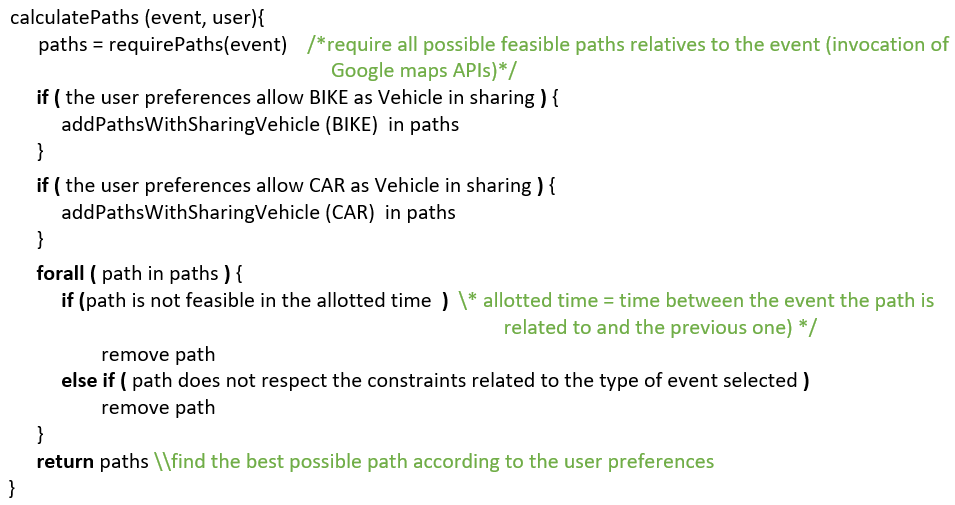
\includegraphics[width=\textwidth]{algorithms/calculate_paths.png}
\end{center}
\end{figure}
\noindent The addPathsWithSharingVehicle method is explained below:
\begin{figure}[H]
\begin{center}
		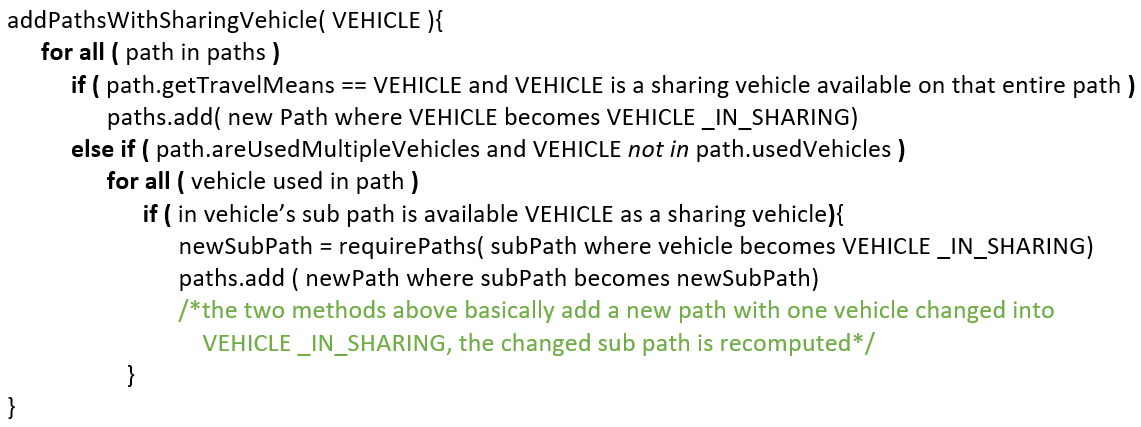
\includegraphics[width=\textwidth]{algorithms/sharing_method.png}
		
\end{center}
\end{figure}


\section{Univocal code}
\label{sect: Univocal code}
	In the registration process the username and the password (sended with the encryption algorithm specified above) are written in the database.\\
Log in operation is required in order to use the functionalities of the system.
\\\\
When login happens the user inserts username and they are sended to the system; the system also obtains the ID device exploiting a GCM's function. In the DB several IDdevices can be associated to the same user, there is a field that marks the ID as mobile (related to phones and tablets) or browser (related to PCs). Browser IDs are deleted periodically. 
\\\\
The system behaves as specified in the flowchart according to the situation:
\begin{itemize}
\item first access: device is not present in the database;
\item login with different device: device is in the database, but it is associated to a different user;
\item login with the same device (not for the first time): a new univocal code is calculated and it will be update on the database.
\end{itemize}
The univocal code is a randomly generated string concatenated to the username (unique). The random string is calculated with the Current Unix Timestamp.
\\\\
The univocal code is sent to the device (a parameter that will be stored locally in the case of a mobile application, a cookie in the case of a browser) and will be used for every interaction with the system: in this way happens the identification of the user. For each request the system takes the univocal code received and the ID of the device and checks in the database if they are related.
\\
\begin{figure}
	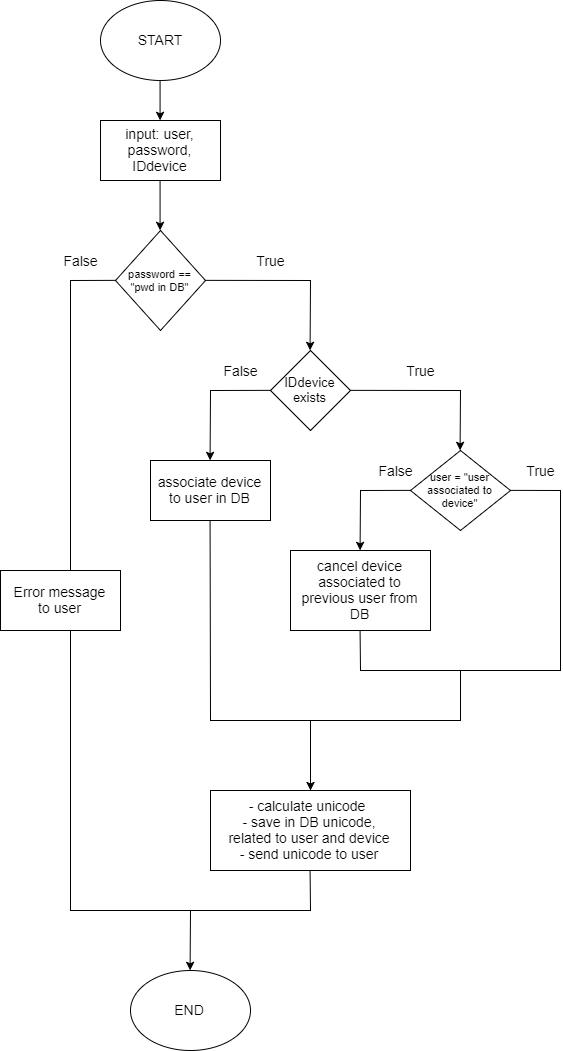
\includegraphics[scale=0.6]{algorithms/unicode_fc.png}
	\centering
	\caption{What happens during the login phase}
\end{figure}


\section{Swap events in the schedule}
\label{sect: Swap events in the schedule}
	The purpose of this algorithm is to check and manage the schedule when an overlapping event is forced into it, maintaining thus a feasible list of scheduled events. \\ \\
To explain it we will use the following terms: 
\begin{itemize}
	\item \textit{ForcedEvent}: The event that is going to be put into the schedule;
	\item \textit{ScheduledEvent}: An event that will be removed from the schedule as a consequence of the ForcedEvent insertion;
	\item \textit{ScheduleList}: A list containing all the scheduled events for a specific day;
	\item \textit{OverlappingList}: A list containing all the overlapping events for a specific day.
\end{itemize}
\newpage
\noindent The algorithm works in this way:
\begin{enumerate}
	\item Checks if there are ScheduledEvents with: \\ \textit{startingTime(ScheduledEvent) \textless startingTime(ForcedEvent) \textless endingTime(ScheduledEvent)} \\ or \\ \textit{startingTime(ScheduledEvent) \textless endingTime(ForcedEvent) \textless endingTime(ScheduledEvent)} \\
or \\ \textit{startingTime(ForcedEvent) \textless startingTime(ScheduledEvent) AND \\endingTime(ScheduledEvent) \textless endingTime(ForcedEvent)}. \\
	If the condition results True for one or more scheduled events, it removes them from the schedule and puts them in the overlapping list;
	\item Computes the travel of ForcedEvent, depending on the previousLocation inserted or, if a previous starting location for the travel is not defined, on the location of the previous ScheduledEvent;
	\item If the travel used to reach the ForcedEvent requires a departure time that is less than the previous ScheduledEvent ending time, the previous ScheduledEvent is removed from the ScheduleList and added to the OverlappingList;
	\item Repeats 2 and 3 until a ScheduledEvent considered is still feasible after the insertion of the ForcedEvent;
	\item Recomputes the travel of the ScheduledEvent that follows ForcedEvent. If that ScheduledEvent's location is not reachable in time for its starting time anymore, this ScheduledEvent is removed from the ScheduleList and added to the OverlappingList;
	\item Repeats 5 until the ScheduledEvent following ForcedEvent in the ScheduleList is still a feasible one after the recomputation of its travel;
	\item ForcedEvent has been successfully inserted in the schedule.
\end{enumerate}

\section{Flexible breaks}
\label{sect: Flexible breaks}
	The purpose of this algorithm is to check if a flexible break inserted is respected by the events present in the schedule. \\ \\
To explain it we will use the following terms: 
\begin{itemize}
	\item \textit{BreakList}: a list containing all the events that overlap, even partially, with the flexible break time slot;
\end{itemize}
The algorithm works in this way:
\begin{enumerate}
	\item Puts in BreakList all the scheduled events that take place during the allotted break time slot, even if partially;
	\item Checks if at least one of the spare time slots between an event of BreakList and the following one (including travels) is larger enough to include the break event;
\end{enumerate}	
SPECIAL CASE: if only one event is present in BreakList, the algorithm must check that the remaining spare time in the slot is larger enough to allocate the break event.

\section{Periodical events}
\label{sect: Periodical events}
	The purpose of this algorithm is to manage the creation of periodical events. \\ \\
The algorithm works in this way: when a periodical event is inserted, a number of events is generated in order to cover a span of one year, e.g. if an event like "Friday lunch with parents" with a weekly periodicity is created, 52 different events will be created.
To better understand the reasoning behind this, take a look at section \ref{sect:Other design decisions}.

